\documentclass[conference,a4paper]{IEEEtran}
\usepackage[T1]{fontenc}
\usepackage{cite}
\usepackage{amsmath,amssymb}
\usepackage{booktabs,tabularx}
\usepackage{graphicx}
\usepackage{url}
\usepackage[hidelinks]{hyperref}
\hypersetup{pdfauthor={},pdftitle={Hazardous-Object Retrieval: Mobile Manipulation Architecture and Coordination Study}}
\graphicspath{{figures/}}
\newcommand{\code}[1]{\texttt{#1}}
\begin{document}
\title{Hazardous-Object Retrieval: Mobile Manipulation Architecture and Coordination Study}
\author{\IEEEauthorblockN{Anonymous Authors}}
\maketitle
\begin{abstract}
Retrieving an object from a potentially hazardous area requires coordinated perception, mobility and manipulation. We present HazBot, a Raspberry Pi-centered mobile-manipulation architecture with four subsystems: LiDAR navigation, differential wheel drive, native camera inference and an articulated gripper. A direct CSI camera and separate drive, arm and sensor-controller paths support a seven-phase reference retrieval mission with explicit handoff prerequisites. Ball-based simulated control provides a nonhazardous task context; evaluation comprises three offline studies rather than physical mission trials. Exhaustive analysis of the isolated wheel-command branch covers 261,121 input pairs, identifies magnitude loss in direction-only translation and finds 1,020 mixed-zero pairs that request no new command. Two URDF links give a 0.200\,m shoulder-to-wrist bound; 68,921 joint samples characterize the ideal wrist envelope. The full reference coordinator produces no violations of the specified command contracts across 28,672 phase--observation pairs; removing individual guard groups exposes counterexamples. The contribution is an implementation-grounded architecture and coordination study that identifies gateway, feedback and calibration requirements for subsequent task-specific retrieval experiments.
\end{abstract}

\begin{IEEEkeywords}
Mobile manipulation, Raspberry Pi, hazardous-object retrieval, embedded vision, subsystem coordination, model-based verification.
\end{IEEEkeywords}
\section{Introduction}
Moving a suspect object away from people combines several robotics problems: locating a candidate, navigating toward it, positioning a gripper, transporting the object, and confirming its release. Each component can function in isolation while the complete task remains unreliable. A valid detection may arrive after its target has moved; a motion command may lose its intended magnitude at a serial gateway; an object may lie outside the arm's contact workspace even when the base has reached its navigation goal. The central engineering problem is therefore the relationship between subsystem evidence and permission to act.

Mobile robots have been developed for nuclear environments~\cite{bird2022vega}, and compact mobile manipulators demonstrate the value of integrating mobility and reach~\cite{kemp2022stretch}. HazBot addresses an accessible embedded implementation of this integration. Its central Raspberry Pi connects four functional subsystems: navigation, wheel control, visual inference, and robotic manipulation. Local perception keeps image interpretation on the robot, while dedicated embedded controllers separate sensor acquisition and actuator signaling from mission-level decisions.

We frame the application as retrieval of designated objects from a potentially hazardous area. A task specification determines which objects may be handled and where they should be deposited. Visual recognition proposes a candidate; authorization determines whether handling is permitted. This distinction accommodates task-specific detectors without treating appearance as evidence of chemical, radiological, or biological properties. Ball-based simulated control provides a nonhazardous task surrogate for the present study.

The paper makes three contributions. First, it specifies a Pi-centered four-subsystem architecture with explicit physical interfaces and separate drive, arm, and ranging controller paths. Second, it defines a seven-phase reference coordinator with observable prerequisites for mobility--manipulation handoffs. Third, it provides reproducible model and source analyses that connect these prerequisites to wrist geometry and actual command semantics. The evaluation establishes properties of the discrete coordinator and source models; physical retrieval performance remains a separate measurement problem. This scope permits precise results without borrowing detector accuracy, payload, or mission-success figures from unrelated systems.

\begin{figure*}[t]
\centering
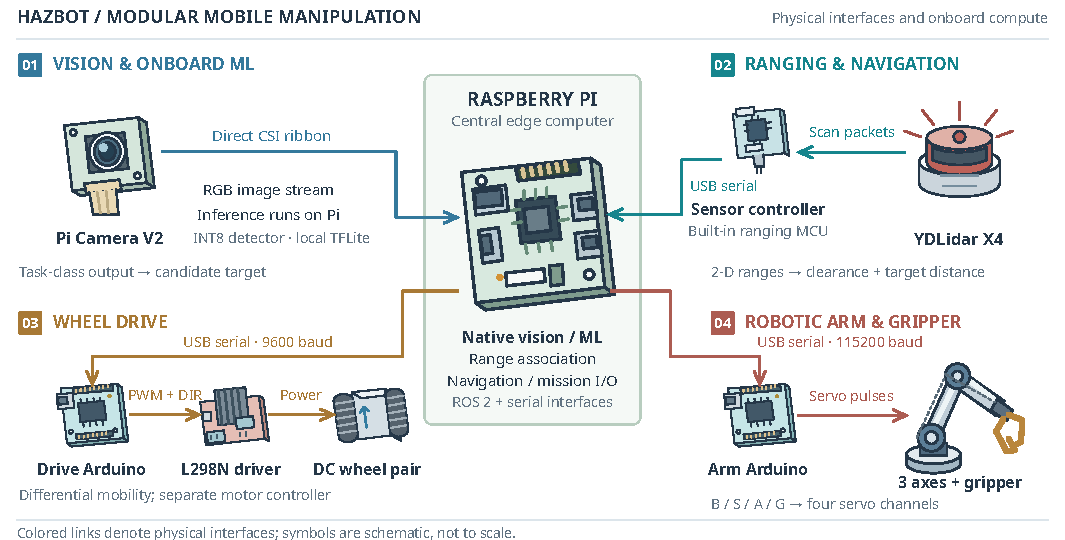
\includegraphics[width=\textwidth]{hazbot_architecture.pdf}
\caption{HazBot's four-subsystem architecture. The Raspberry Pi performs onboard computation and interfaces with a direct CSI camera, a LiDAR sensor controller, a dedicated drive Arduino, and a separate arm Arduino. Glyphs identify functional hardware; the drawing is a topology rather than a scale assembly. The complete mission coordinator is evaluated as a reference model.}
\label{fig:architecture}
\end{figure*}

\section{Related Work}
\subsection{Application and Mobile Manipulation}
Vega provides a relevant hazardous-environment precedent: Bird \emph{et al.} describe a small ground robot for nuclear decommissioning with engineering directed toward its operating environment~\cite{bird2022vega}. Its application illustrates the importance of environment-specific qualification. Stretch combines a differential mobile base and compact manipulator, supported by design analysis and physical task demonstrations~\cite{kemp2022stretch}. HomeRobot treats navigation, recognition, grasping and placement as a connected mobile-manipulation problem with distinct simulation and real-world evaluation components~\cite{yenamandra2023homerobot}. These studies motivate HazBot's complete retrieval sequence and the coordination of its sensing and actuation modules.

\subsection{Embedded Integration and Coordination}
ROS 2 provides a common communication and software framework for distributed robotic components~\cite{macenski2022ros2}. Nav2~\cite{macenski2020marathon2} and SLAM Toolbox~\cite{macenski2021slamtoolbox} provide established navigation and mapping capabilities. These components supply reusable interfaces for integrating onboard observations and motion requests. Edge-device detector evaluations further motivate explicit characterization of model and device choices~\cite{alqahtani2026edge}, including the configuration used for local inference.

Command arbitration and sensor-dependent stopping are established in systems such as \code{twist\_mux} and Nav2 Collision Monitor~\cite{twistmux,nav2collision}. HazBot focuses on the connection between a four-subsystem embedded design, retrieval-phase prerequisites and reproducible characterization of the particular geometry and gateways that implement those interfaces. The reference coordinator makes this integration inspectable before a physical mission benchmark is attempted.

\section{System Architecture}

\begin{table}[t]
\caption{Four Subsystems and Their Pi Interfaces}
\label{tab:interfaces}
\centering\footnotesize
\begin{tabularx}{\columnwidth}{@{}lX@{}}
\toprule
Subsystem & Connection and responsibility \\
\midrule
Vision / ML & CSI camera directly to Pi; local TFLite inference. \\
Navigation & LiDAR sensor controller and USB--UART path; ranging data consumed on Pi. \\
Wheel drive & USB serial, 9600 baud, to drive Arduino; PWM/direction through L298N. \\
Manipulator & Separate USB serial, 115200 baud, to arm Arduino; four servo channels. \\
\bottomrule
\end{tabularx}
\end{table}

\subsection{Central Computer and Physical Interfaces}
Figure~\ref{fig:architecture} shows the hardware interfaces; Fig.~\ref{fig:workflow} connects sensing and Pi processing to command generation through the reference coordinator. The analyzed configuration comprises a Pi Camera V2, YDLIDAR X4, L298N differential drive and servo arm; Table~\ref{tab:interfaces} lists the interfaces. A workstation supports visualization without hosting the native detector. Figures~\ref{fig:prototype} and~\ref{fig:front} show the prototype and laptop; the local display uses GPIO and the camera a white CSI ribbon. Figure~\ref{fig:dashboard} documents the command surfaces, not live-system performance.

\HazBotWorkflowFigure

% Original photograph with compact numbered markers; key stays in the caption.
\IfFileExists{figures/hazbot_prototype.pdf}{%
\begin{figure}[t]
\centering
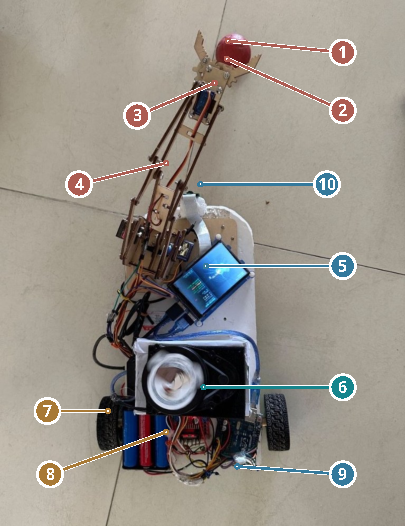
\includegraphics[width=0.78\columnwidth]{hazbot_prototype.pdf}
\caption{Physical HazBot prototype. Markers identify: 1, ball surrogate; 2, gripper; 3, servo; 4, arm linkage; 5, Raspberry Pi with GPIO-mounted display; 6, LiDAR; 7, drive wheel; 8, battery cells; 9, control electronics; 10, camera at the end of the white CSI ribbon.}
\label{fig:prototype}
\end{figure}
}{}

\IfFileExists{figures/hazbot_front.pdf}{%
\begin{figure}[t]
\centering
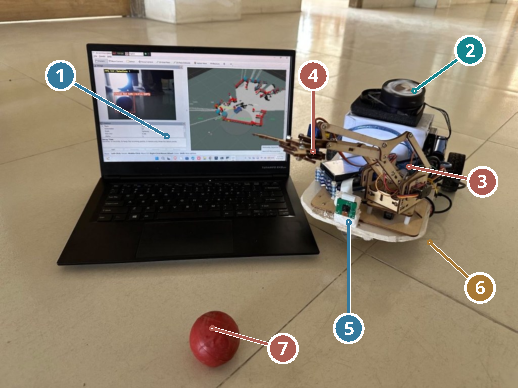
\includegraphics[width=\columnwidth]{hazbot_front.pdf}
\caption{Front view with laptop visualization. Markers identify: 1, laptop visualization; 2, LiDAR; 3, arm linkage; 4, gripper; 5, CSI camera; 6, mobile base; 7, ball surrogate.}
\label{fig:front}
\end{figure}
}{}


\subsection{Navigation and Wheel Control}
The LiDAR controller acquires ranges and sends packets to the Pi over USB. Host navigation uses scans for route clearance and target-distance association. ROS 2 mapping components are available, but map quality and localization error are not measured here.

The wheel Arduino drives the motor bridge independently of the arm controller. For an ideal differential base, wheel radius $R$ and track $b$ relate desired body velocity $(v,\omega)$ to wheel angular rates:
\begin{equation}
\dot\phi_L=\frac{v-b\omega/2}{R},\qquad
\dot\phi_R=\frac{v+b\omega/2}{R}.
\label{eq:drive}
\end{equation}
The model uses $R=0.033$\,m and $b=0.210$\,m. Realizing Eq.~\ref{eq:drive} requires a gateway that preserves wheel-rate semantics; the command study tests this condition.

\subsection{Vision and Native Inference}
The direct CSI path configures $640\times480$ RGB capture and a two-thread TFLite interpreter for an INT8 detector. Its tennis- and cricket-ball labels provide task surrogates. Hazard-related classes require a corresponding dataset and evaluation. Model weights are absent from the analyzed artifacts; accuracy and execution time are not reported.

A detection record should carry class, confidence, image position and age. Metric approach also requires range associated with the same target and frame. Class acceptance and freshness are distinct: a confident stale record cannot authorize approach. Task authority supplies handling permission; confidence establishes neither material identity nor authorization.

\subsection{Robotic Hand and Arm}
The arm has base yaw, shoulder pitch and elbow pitch, a fixed wrist and a separately actuated gripper. Its dedicated Arduino drives four servo channels, not four positioning joints. Existing commands include a preset pickup sequence; the seven-phase coordinator is a separate executable reference model. Separate drive and arm boards retain distinct serial protocols and pin assignments.

\section{Retrieval Coordination and Analysis Method}
Figure~\ref{fig:methodology} links the mission specification, URDF chain and actuator gateways to three offline studies: coordinator verification, wrist geometry and command semantics. Their evidence identifies integration requirements for subsequent physical trials.

\HazBotMethodologyFigure
\subsection{Mission and Evidence Contracts}
The reference mission has seven phases (Fig.~\ref{fig:mission}): SEARCH authorizes a candidate; APPROACH reaches its pickup region; DOCK transfers control from base to arm; GRASP secures the object; CARRY transports it with the arm stowed; PLACE releases it at the deposit region; and COMPLETE requires a release indication.


\begin{figure*}[t]
\centering
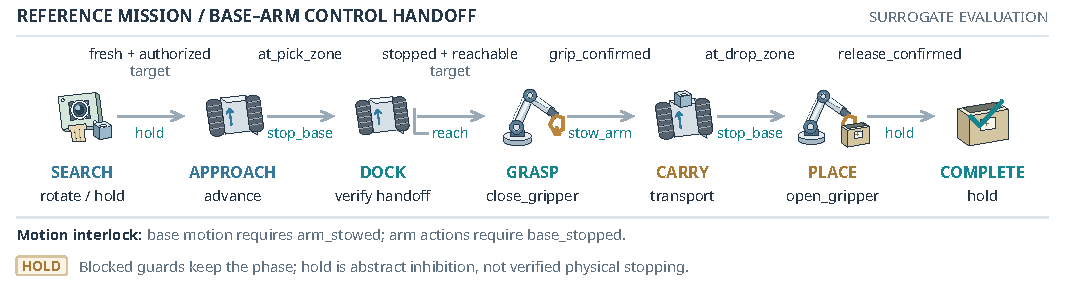
\includegraphics[width=\textwidth]{hazbot_mission.pdf}
\caption{Seven-phase reference retrieval mission. Conditions summarize the handoff evidence; complete command predicates are defined in the text and executable model. A failed prerequisite requests HOLD at the current phase. The strip depicts the coordination specification, rather than a measured physical trajectory.}
\label{fig:mission}
\end{figure*}

Let $T$ denote an authorized, fresh target; $S$ a fresh, usable scan; $C$ a clear route; $A$ a stowed arm and $B$ a stopped base. The principal command contracts are
\begin{align}
\text{base motion} &\Rightarrow S\land C\land A,\label{eq:baseguard}\\
\text{target approach} &\Rightarrow T,\\
\text{arm motion} &\Rightarrow B.\label{eq:armguard}
\end{align}
Reach and closure additionally require $T$ and wrist reachability; release requires the deposit region and a grip indication. The controller also requires scan health during docking, grasping and placement. A failed prerequisite emits HOLD without advancement. HOLD inhibits active motion and needs an explicit actuator-boundary stop. Target acquisition and release may advance phase while emitting HOLD. A stop request does not establish $B$: deployment requires measured base-rest feedback and a defined confirmation rule.

The abstract observations comprise twelve Boolean values: target authorization and freshness; scan freshness and usability; route clearance; arm stowage; base stopped; wrist reachability; pickup-region arrival; grip confirmation; deposit-region arrival and release confirmation. Each has a specific role in the interface but this discrete model does not generate these observations from physical sensors. In particular, grip and release indications are input assumptions, not inferred force or contact measurements.

\subsection{Bounded Reference-Model Verification}
The verification procedure in Fig.~\ref{fig:verification} enumerates every observation valuation at every phase: $7\times2^{12}=28{,}672$ phase--observation pairs per policy. No valuations are pruned. A separate admissibility oracle checks the output action against Eqs.~\ref{eq:baseguard}--\ref{eq:armguard} and the target, reach and placement conditions. Breadth-first exploration establishes phase reachability and extracts shortest-prefix counterexamples. Three ablations remove the base--arm interlock, target authorization or scan-age requirement from the controller while retaining the full oracle. This design tests whether each omitted condition creates a concrete contract violation.

All Boolean valuations are retained, including physically inconsistent combinations. Counts therefore describe the specification domain, not robot failure probabilities. A nominal trace checks progression to COMPLETE under admissible observations; neither it nor existential phase reachability establishes physical mission success.

\HazBotVerificationFigure

\subsection{Source-Derived Wrist Geometry}
Figure~\ref{fig:workspace} connects arm geometry to the docking prerequisite. From the URDF chain, the shoulder lies at $(0.100,0,0.155)$\,m in the base frame and both positioning links have length $L_1=L_2=0.100$\,m. The zero pose has a vertical upper link and horizontal forearm. The figure uses $q_1=q_b$, $q_2=q_s$, and $q_3=q_e$. For yaw $q_b$, shoulder angle $q_s$, and elbow angle $q_e$, the wrist origin is
\begin{align}
r &=L_1\sin q_s+L_2\cos(q_s+q_e),\\
x &=0.100+r\cos q_b,\quad y=r\sin q_b,\\
z &=0.155+L_1\cos q_s-L_2\sin(q_s+q_e).
\label{eq:fk}
\end{align}
We sample 41 values, including both bounds, for each positioning joint. The declared bounds are $q_b\in[-1.5708,1.5708]$, $q_s\in[-0.5,2.6179]$, and $q_e\in[-1.5708,2.6179]$\,rad. An independent homogeneous-transform implementation evaluates the URDF chain at 1,000 seeded random poses and 13 special poses. Agreement checks numerical implementation, while the grid characterizes the ideal wrist envelope. The wrist origin is not a calibrated grasp contact point; collision, load, compliance and stability constraints are not represented.

\begin{figure}[t]
\centering
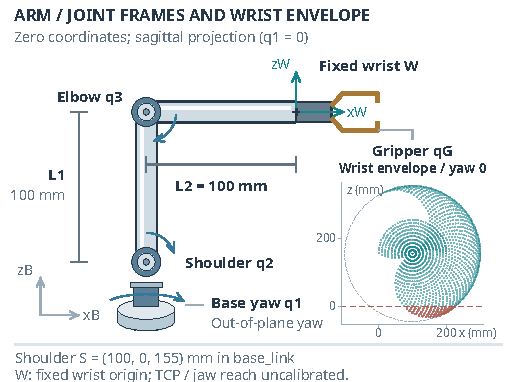
\includegraphics[width=\columnwidth]{hazbot_arm_geometry.pdf}
\caption{Source-derived arm geometry at zero joint coordinates, with joint axes and fixed wrist origin. The small inset shows 1,681 zero-yaw wrist samples, the link-sum bound, and modeled ground exclusions. Samples describe ideal geometry rather than calibrated contact positions or collision-free grasps.}
\label{fig:workspace}
\end{figure}

\subsection{Command-Interface Characterization}
Using Python's abstract syntax tree, we isolate the \code{SET:} branch of the actual wheel gateway and replace only the transport sender with an in-memory recorder. All integer pairs $(l,r)\in[-255,255]^2$ are executed and compared with an independently specified sign partition. The arm gateway's pure angle mapper is evaluated for five accepted aliases over 451 inputs from $-90$ to $360$, checking clamps and reversals. The elbow has two aliases, so this represents four actuator channels. No ROS constructors, sockets, motor servers or hardware launchers are executed. Source hashes, settings, CSV outputs and validation records bind the results to the analyzed implementation.

\section{Results}
\subsection{Mission Handoffs}
Figure~\ref{fig:verification} combines the verification procedure, ablation counts and phase-reachability results.
% Generated by experiments/verify_hazbot_mission.py; values come from computed results.
The full reference coordinator admits 0 contract-violating commands among 28,672 phase--observation pairs. All 7 phases are reachable with 13 unique phase edges (including self-loops) and a shortest completion depth of 6 transitions. A separate 11-step nominal witness exercises all 9 action types and reaches COMPLETE.

Removing the base--arm interlock produces 480 violating pairs; removing target authorization produces 128 and removing scan-age checks produces 288. Their shortest counterexample prefixes contain 1, 2, and 1 observations respectively. For example, the interlock ablation permits SEARCH rotation while the arm is not stowed. These counts demonstrate guard sensitivity over the enumerated domain and they are not observed mission failure rates.


\subsection{Geometric Envelope and Docking}
The $41^3$ grid contains 68,921 wrist poses with a link-sum bound of $0.200$\,m. Sampled height spans $-0.0316$ to $0.3549$\,m: 2,747 poses lie below modeled ground and 66,174 on or above it. These are joint-grid counts, not Cartesian volumes; above-ground poses may still violate collision or stability constraints.

Independent forward-kinematics implementations agree over 1,013 poses within $6.8\times10^{-17}$\,m, validating numerical implementation rather than mechanical accuracy. Docking requires calibrated contact geometry and target pose; the ideal wrist envelope is a starting point for that calibration.

\subsection{Wheel and Arm Command Semantics}
All 261,121 wheel pairs match the sign partition. Each nonzero sign quadrant maps 65,025 pairs to one direction request, discarding magnitude. Only $(0,0)$ requests stop; 1,020 mixed-zero pairs make no sender call. Thus, a stationary-wheel/moving-wheel request is not preserved. The absence of a command request is distinct from a stop request; neither establishes subsequent actuator behavior.

This limits the realization of Eq.~\ref{eq:drive}: approach and docking require deliberate discrete primitives or a magnitude-preserving, calibrated wheel-rate path. No physical speed error is measured.

All 2,255 arm cases match the independent clamp/reversal specification. The base-yaw command retains direction, shoulder and elbow mappings reverse direction, and gripper commands are clamped to their declared range. Mapping commands to modeled angles still requires calibration. All 29 geometry/interface checks pass. The two detector labels confirm only the surrogate configuration, not recognition accuracy.

\section{Discussion and Application Development}
The architecture connects object retrieval through explicit subsystem evidence: vision proposes a candidate, task authority permits handling, navigation establishes a pickup region, the base confirms rest, and manipulation confirms grip and release. The mission model exposes these obligations where hardware feedback remains to be developed. Its nominal trace demonstrates logical progress under stated assumptions, while source analysis identifies what the actuator gateway can express.

The next application step is to instantiate these observations with measured quantities. This requires a task-specific visual dataset and held-out recognition results; calibrated camera--LiDAR--arm frames and contact geometry; feedback for base rest, grip, and release; and timed physical runs covering navigation, pickup, transport, and deposit. Sensor-age limits must follow measured acquisition and transport behavior. Force, payload, containment, and environmental compatibility must be evaluated for the designated object class. A general RGB category detector cannot establish an unknown material's hazardous properties.

The results establish source and model properties; physical obstacle avoidance and hazardous-environment suitability require application trials. Nonhazardous surrogates support the initial benchmark, followed by object- and environment-specific qualification as illustrated by prior systems~\cite{bird2022vega,kemp2022stretch}.

\section{Conclusion}
HazBot organizes navigation, wheel control, native visual inference, and robotic manipulation around a Raspberry Pi. A seven-phase reference mission makes the transitions from target selection to retrieval and placement explicit. Source-derived analysis links those transitions to a bounded wrist envelope and actual serial-gateway behavior, including magnitude reduction and mixed-zero command omissions. The resulting artifact provides a concrete basis for improving embedded mobile manipulation and developing task-specific hazardous-object retrieval, with subsequent physical evaluation tied to clearly defined observations and interfaces.

\section*{Acknowledgment}
The authors acknowledge the ROS 2, Nav2, and open-source robotics communities for their publicly available software and technical documentation. ChatGPT, a large language model developed by OpenAI, assisted literature discovery and synthesis, study design, code development, analysis, manuscript drafting, and editing. The authors are responsible for reviewing and approving the content and for the accuracy and integrity of the submitted work.
\bibliographystyle{IEEEtran}
\bibliography{references}
\end{document}
